\documentclass[12pt,a4paper,final]{article}
\usepackage[latin1]{inputenc}
\usepackage{amsmath}
\usepackage{amsfonts}
\usepackage{amssymb}
\usepackage{graphicx}
\usepackage{varioref}
\usepackage[english]{babel}
\usepackage[latin1]{inputenc}
%\usepackage[leqno]{amsmath}
\usepackage{here}
\usepackage{textcomp}
\usepackage{mathrsfs,euscript}
\usepackage{booktabs}
\usepackage{dcolumn}
\usepackage{epsfig}
\usepackage{upref}
\usepackage{paralist}
\usepackage{calc}
\usepackage{setspace}
%\usepackage[parfill]{parskip}
\usepackage[left=3.5cm,right=3.5cm,top=2cm,bottom=2cm]{geometry}
\usepackage[longnamesfirst]{natbib}
\bibliographystyle{plainnat}
%\usepackage{biblist}
%\usepackage{chicago}
%\bibliographystyle{chicago}
\usepackage{graphicx,float}
\usepackage{graphics}
\usepackage{multicol}
\usepackage{float}
\usepackage[normalem]{ulem}
\author{Eliab G. Luvanda}

\title{Construction of Business Cycle Indicators \\
\textbf{REPORT} \\
Submitted to \\
\textbf{Tanzania Revenue Authority (TRA)}}

\date{March 7, 2016}
\begin{document}

\maketitle

\newpage
\pagenumbering{roman}
\tableofcontents

\listoffigures

\listoftables

\newpage
\pagenumbering{arabic}
\section{Introduction}

\subsection{Background}
Business cycles are output fluctuations that involve movements in GDP overtime in alternating periods of expansion in economic activity (boom) and contraction in economic activity (recession). GDP/output being a base of tax revenue, business cycles are usually associated with fluctuations in tax revenue.  The upwardand downward swings in macroeconomic variables include GDP growth of domestic  and external economies, inflation, exchange rate, credit to the private sector, investment levels and more others.  These variables need to be monitored to detect their short and medium term influence on revenue collection. This study estimates business cycles and  examines how the cycles influence tax revenue, and more specifically to what extent business cycles influence flucuations in tax revenue in Tanzania.  

Business cycles in this case means fluctuation in output/GDP, which is the overall tax base, and also fluctuations in sectoral output/GDP, constituting bases for different taxes. In this case, tax revenue is defined in a way that excludes non-tax revenue.  Regarding tax revenue, this study covers tax revenue from the major sectors: agriculture, industry and services. In terms of time coverage, the period from 1966 to 1994 has been covered by the study for the estimation of business cycles. The reason for this is that a reasonable long time coverage is needed for obtainint reliable estimates of business cycles.  Given the fact that the main  tax categories for which the data is avalable for the entire 1966-2014 period are income tax, import and excise duties, and others (as a tax category), business cycles have been estimated for only those broad tax categories. 

\subsection{Objective of the assignment}
In view of the fact that business cycles have a significant impact on tax revenue, this study estimates business cycles and examines how they are related  to revenue collection performance.  That is the main objective of this study.  The specific objectives include the following:

\begin{compactenum}[1)]
\item Examine the nature, main features and causes of business cycles in Tanzania and the associated reasons for their occurrence. 

\item	Analyze economic sectors' behavior and  sectoral revenue data and determine the more responsive sectors in terms of upward and downward movements as well as their impact on revenue. This objective requires examining the behavior of economic sectors (such as agriculture, manufacturing, services, mining etc); and examine how the sectoral performance influence tax revenue.  More specifically, this objective requires the study to carry out the following:

\begin{compactenum}[(i)]
\item	Examine the sectoral performance (in terms of output) trends, and relative contribution of sectors to GDP;

\item	Examine the sectoral performance over the business cycle.   

\item Examine the extent to which tax revenue responds to movements in sectoral output. 

\end{compactenum}

\item 	Examine the extent to which tax revenue responds to both long term and cyclic movements of GDP/output. 

\item Prepare a model report on Tanzania business cycles linking with tax collection.  This will involve coming up with a report, which among other things, will include a model linking tax revenue with business cycles.
 
\end{compactenum}




\section{Methodology}
The specific objectives of the study have guided the design of the  methodology. This section explains the study methododology  and how the different aspects of the methodology do address the specific objectives of the study.

\subsection{Literature Review}

Both theoretical and empirical literature related to business cycles and the behaviour of tax revenue over the business cycle have been reviewed.  The main aim of this review was to explore the theory behind business cycles in relation to tax revenue and guide the choice of analytical techniques for carrying out the assignment.

\subsection{Data Collection}

Secondary data has been used. Time series data for macroeconomic variables (including tax revenue) has been obtained from official publications (database kept) by the Bank of Tanzania (BOT), the National Bureau of Statistics (NBS), and Tanzania Revenue Authority (TRA).  The International Financial Statistics (IFS) was another source of time series data for the variables.  Qualitative information has been obtained from the publications.

\subsection{Data Analysis}

The Prescott-Hodrick filter has been used to estimate the trend and cyclic components of GDP/output other macroeconomic variables such as tax revenue, inflation, government expenditure and money supply. Kendall's correlation coefficients have been computed to determine which variables are pro-cyclic and whivh variables are counter-cyclic. Cointegration test has been carried out and econometric models have been estimated to examine the relationsip between output and tax revenue.

\subsubsection{Estimation of Trend and Cylic Components of Macroeconomic Variables}

Standard filters such as the Hodrick - Prescott (HP) and Baxter King (BK) filters are commonly used to estimate the trend and cyclic components of the variables.  This study uses the Hodrick - Prescott filter, the most commonly used filter in the business cycle studies.

\subsubsection*{Decomposition of Time Series into Trend and Cyclical Components}

A macroeconomic time series   is composed of two main components: (1) the permanent (or secular) component $y_t^p$ , and (2) the transitory component  $y_t^c$. Thus, a macroeconomic variable can be represented by the following simple model:

\[ y_t = y_t^p + y_t^c \]

where $y_t$  is logarithm of actual observation, $y_t^p$  is a trend or secular component and $y_t^c$  represents deviations from trend or a cyclical component.  Stochastic detrending methods can be used to estimate the trend and cyclic components of macroeconomic variables. The most popular among the stochastic detrending methods is the Hodrick Prescott  (hereafter referred to as HP) (1980) filter.  The other and more recent is the Baxter--King (1995) filter. The HP trend for a variable $y_t$ (in logarithmic form) is found by minimizing the following function:

\[ \sum_{t=1}^T\left( y_t - y_t^{trend}\right) ^2 + \lambda \sum_{t=2}^{T-1} \left[ \left( y_{t+1}^{trend} - y_t^{trend}\right) -\left( y_t^{trend} - y_{t-1}^{trend}\right)  \right] \]

The idea behind this equation is to minimize the sum of two components.  The first component is the sum of squares of the deviation of the actual value of a variable from its trend value.  The second is the sum of squares of changes in the trend growth.  A series of trend values that gives the minimum value of the equation is the HP trend or filter.
A parameter, $\lambda$, controls the degree of smoothness in the HP trend.  On the one hand, a smaller value of $\lambda$ reduces the importance of change in trend growth.  For $\lambda = 0$, a minimum value of the equation is given by selecting the trend value equal to the actual value of the variable.  In this case, there cannot be deviations from trend.  On the other hand, a very high $\lambda$ diminishes the significance of the first component.  In the limit, a smooth deterministic trend yields the minimum of the total sum, and the cyclical component of a variable will be large. 

To get a `reasonable' variable trend, one must choose an intermediate value of $\lambda$.  Hodrick and Prescott (1980) recommend $\lambda = 1600$ for quarterly data, and $\lambda = 100$ for annual data.  However, Ravn et al (1997) recommend $\lambda = 6.75$ for annual data. Once a trend component, has been estimated, the cyclical component of the variable can be obtained by subtracting the trend value from the actual observations of the variable; that is, $y_t^c = y_t - y_t^p$. 

Once the trend and cyclic components have been estimated, they are usually plotted on a graph from which one can study the pattern of long term movement of the variable, and the pattern of cyclic movement/fluctuations of the variable.



\subsubsection{Computation of Correlation Coefficients and Variances}

Kendall's correlation coefficients between the cyclic component of output/GDP (as a reference variable) and cyclic components of other macroeconomic variables (including tax revenue) have been computed.  The correlation coefficients  are used to determine whether the other macroeconomic variables are  procyclical (the cyclic component of the variable move in the same direction as the cyclic component of output/GDP); or whether the other macroeconomic variables are counter-cyclical (the cyclic component of the variable move in the different relative to the cyclic component of output/GDP). Variances of the cyclical components of the variables have been computed to measure the volatitilty of fluctuations of the economic variables over the business cycle.

\subsection{Econometric Analysis}

Econometric analysis has been employed to examine the main factors (monetary and real factors) that drive the busines cycles in Tanzania; and to examine whether long term movements in output do influence tax revenue (categories of tax revenue), and whether short term movements over the business cycle in output do influence tax revenue.

\subsubsection{Vector Autoregression (VAR) Model} 

A simple vector autoregression (VAR) model has been estimated and; and it has been used to examine the relative importance of monetary and real factors in explaining the variations in output. More specifically, the following VAR model has been estimated:

\[ Y_t = \Phi_0 +\Phi_1 Y_{t-1} + \ldots + \Phi_p Y_{t-p} + \varepsilon_t \]

where $Y_t$ is a vector of output/GDP and money supply, $\Phi_0$ is a vector of constants, $\Phi_i$ ($i=1,\ldots,p$) are coefficient matrices; and $\varepsilon_t$ is a vector of error terms that are assumed to be independent and identically distributed.

Basically, there are two major sources/causes of business cycles (macroeconomic fluctuations).  These are monetary and real factors. Regarding monetary factors, variations in money supply are said to cause variations in GDP via variations in the interest rate and investment. As for real factors, variations in the levels of real factors such as labor, capital and technical progress that influence aggregate output in the aggregate production function are said to be the main cause of business cycles. Other factors such as weather conditions, fuel prices, and terms of trade which influence the supply side of the econonomy are also considered to be the real factors that drive business cycles.

Granger causality test has been used to examine whether monetary or real factors do influence output. The variance decompostion analysis has been carried out to examine the relative importance of monetary and real factors in explaining the business cycles.

\subsubsection{Cointegration Test}

Cointegration test has been carried out to examine whether there is a long run equilibrium relationship between tax revenue and GDP by sectors.

\subsubsection{Estimation of Simple Econometric Models}

Simple econometric models will be estimated to examine how tax revenue responds to  output/GDP over the business cycle. The following simple model has been estimated:

\[ T_t = \alpha + \beta Y_t + \varepsilon_t \]

where $T_t$ is the logarithm of tax revenue, and $Y_t$ is the logarithm of tax base (GDP). In this case, tax revenue elasticity with respct to the respective tax base has been estimated for the sectors.

\subsection{Software package}
\textbf{R}, an open source programming environment,  has been used for data analysis. 

%\newpage
\section{Main Findings of the Study}

\subsection{Sectoral Perfomance Trends}

In this section, the peformance of the major sectors is examined.  More specically, the section analyses the trends of contribution of the sectors to GDP and tax revenue over time.  The section also examines the growth patterns in terms of both output and revenue generation.

%\newpage
\subsubsection{Contribution of Sectors to GDP}

The services sector contributes the largest share to GDP.  It's share is about 48 percent.  The share has been rising slightly overtime; from 46 percent in 1998 to 48 percent in 2013 (See Figure 1 below). Agriculture is the next important sector in terms of contribution to overall GDP.  Its share in total GDP is about 27 percent.  However, the relative importance of this sector to GDP contribution has been decreasing gradually; from 32 percent in 1998 to 27 percent in 2013.
\begin{figure}[hbt]
\centering
\begin{small}
\caption{Trends of Sectoral Shares in GDP}
\end{small}
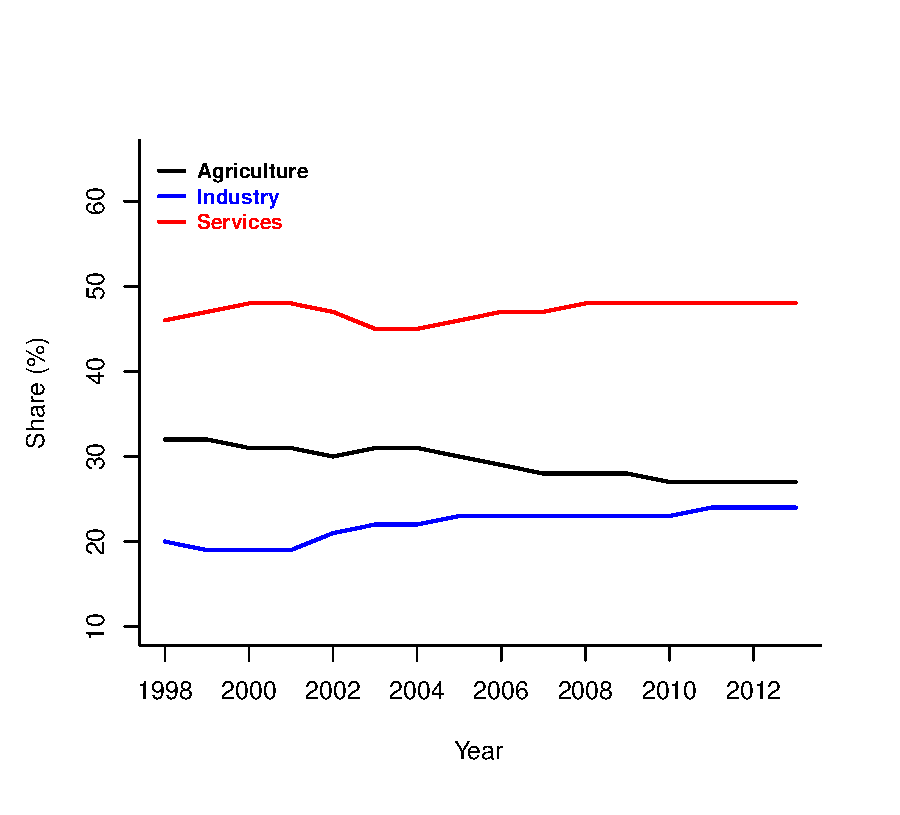
\includegraphics[scale=0.501]{shares.eps} 
\end{figure}

Industry contributes the smallest share; in the sense that it contributes about 24 percent.  However, the share of this sector has been gradually increasing; from about 20 percent in 1998 to about 24 percent in 2013.


\subsubsection{Contribution of Sectors to Tax Revenue}

Just like in the case of contribution by sectors to GDP, the services sector contributes the largest share to tax revenue.  Its share is about 69.8 percent. 

\begin{figure}[h]
\centering
\begin{small}
\caption{Trends of Sectoral Shares in Tax Revenue (\%)}
\end{small}
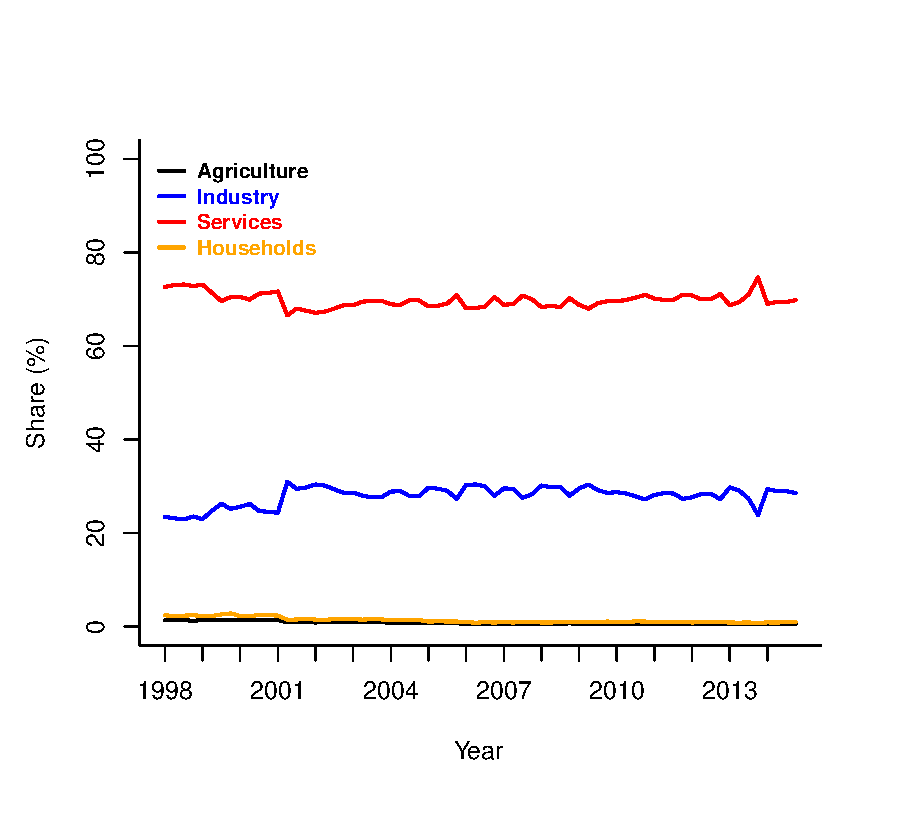
\includegraphics[scale=0.501]{rev_sec_shares.eps} 
\end{figure}

This share has more or less being constant over a decade. Next in importance, but trailing behind by far is the industry sector which, on evarage, contributes about 28.5 percent to tax revenue. The contribution of the agriculture sector to tax revenue is almost neglible, about 0.8 percent.  Households' contribution to tax revenue is about 1.4 percent.

\newpage
Figure 3 below presents trends of revenue generation by sectors. However, it should be noted that because of large differencs in absolute figures of the sectors, the logarithm scale on the vertical axis has to be used for the convenience of comparison.

\begin{figure}[ht]
\centering
\begin{small}
\caption{Trends of Tax Revenue by Sectors}
\end{small}
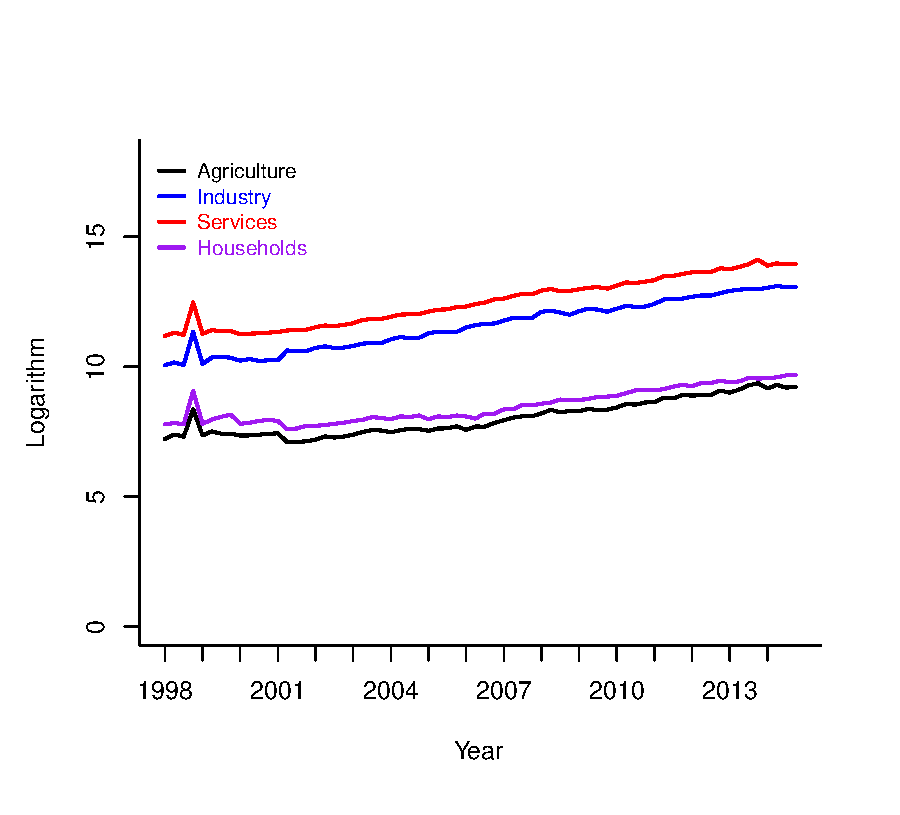
\includegraphics[scale=0.501]{rev_sec_trends.eps} 
\end{figure}

As the Figure shows, generally speaking, tax revenue from all sectors increased over time.  However, estimates of revenue growth for the 1998-2013 period suggest that tax revenue from the industry sectry sector relatively rose at the highest rate of 4.8 percent, followed by the services sector at 4.6 percent\footnote{Estimates of growth rates are presented in Table \ref{tab7} in the Appendix}.   Low growth rates characterised the agriculture and household sectors, with the growth rates of 3.2 percent and 3 percent, respectively.

\newpage
Table \ref{tab1} below presents revenue growth by disaggregated sector for the period 2001 - 2014. As the Table shows, revenue from the financial sector has the highest growth rate, of 6.5. 

\begin{table}[h]
\centering
\begin{small} 
\caption{Revenue Growth per Quarter by Sectors: 2001 - 2014} 
\label{tab1}
\begin{tabular}{l c }
\toprule
\multicolumn{1}{l}{\textbf{Sector}} & \textbf{Mean}\\ 
 \midrule
Agriculture & 4.2\\ 
Mining & 5.4 \\
Manufacturing & 5.0 \\
Electricity & 5.9\\
Construction & 4.1\\
Trade  & 4.4\\
Transport  & 5.0 \\
Hotels & 5.4\\
Financial services & 6.5\\
Real estates & 3.5\\
Education & 4.5\\
Health & 3.8\\
\bottomrule
\end{tabular}
\end{small}
\end{table}

Revenue from mining and hotel sectors also recorded high growth rate of 5.4 percent. Manufacturing and transport sectors also recorded high growth rate of 5 percent.  Revenue from real estates and health sectors grew at low rates of 3.5 percent and 3.8 percent, respectively.

%\newpage
\subsection{Business Cycles}

This Subsection presents estimates of business cycles. A standard Hodrick-Prescott filter has been used to decompose the macroeconomic variables: GDP, inflation,  money supply - broadly defined (M2), government expenditure and tax revenue into trend and cyclic components. As it has been mentioned in the methodology Section, business cycles for the three broad categories of tax revenue: (1) income tax, (2) import and excise duties, and (3) other taxes have been estimated because the data covering the 1966 - 2013 period is available only for these broad categories, rather than for the more disaggregated categories of tax revenue.

\subsubsection{GDP}

Figure 4 below presents the thrend and cyclic components of real GDP. A closer examination of the Figure reveals that Tanzania experienced 3 main cycles between 1966 and 1992, and mild economic fluctuations therefater. 

\begin{figure}[ht]
\centering
\begin{small}
\caption{Trends and Cyclic Components of Real GDP}
\end{small}
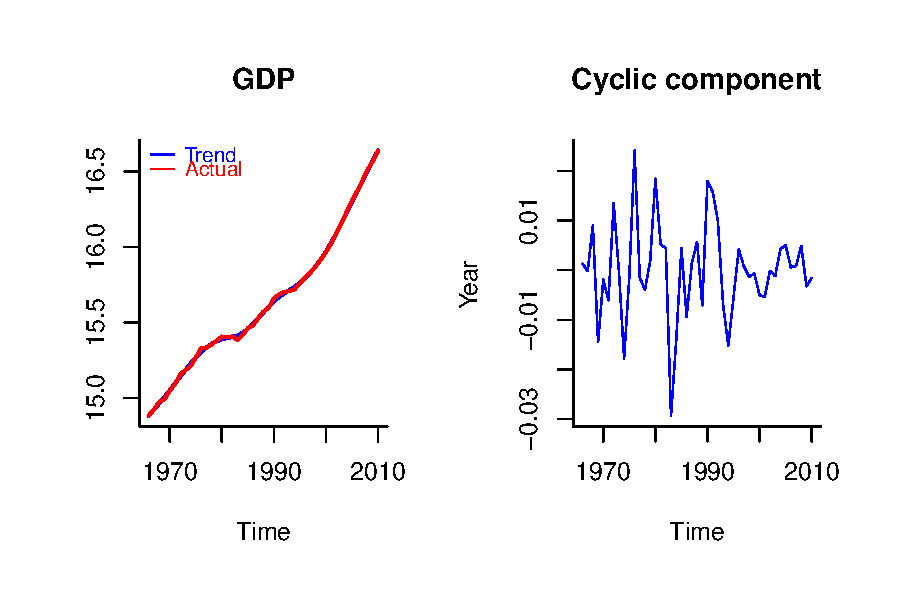
\includegraphics[scale=0.601]{gap_comp.eps} 
\end{figure}

The first major business cycle over the study period occured from 1966 to 1972.  This cycle took 6 years.  The second major cycle occured between 1972 and 1976, and it lasted for approximately 4 years. The last major business cycle, and actually the longest one occured between 1976 and 1992, and it lasted for approximately 16 years. The deviation of actual GDP from trend was at its peak in 1972, when the economy recorded a 6.5 percent growth rate. A deep recession occured in 1983, when the economy recorded a negative growth rate of 2.4 percent, the lowest growth rate ever in the post-independence Tanzania's history.

\subsubsection{Money Supply - Broadly Defined (M2)}

Figure 5 presents an estimate of the cyclic component of money supply - broadly defined (M2). On the right panel of the Figure a cyclic component of GDP is presented for comparison.

\begin{figure}[ht]
\centering
\begin{small}
\caption{Cyclic Component of Money Supply}
\end{small}
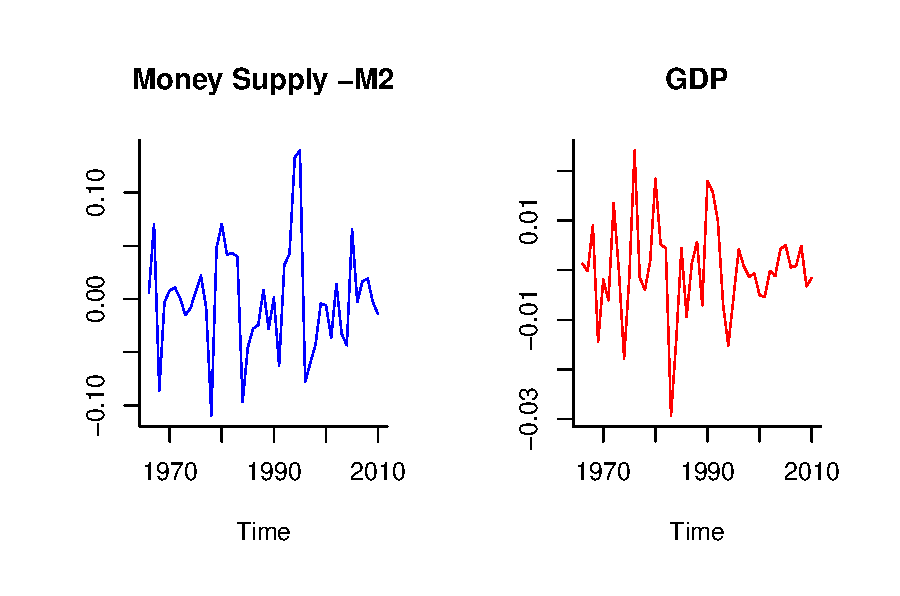
\includegraphics[scale=0.601]{money_supply.eps} 
\end{figure}

Just like in the case of GDP, money suply is characterized by 3 business cycles between 1966 and 1995, and relatively milder fluctuations thereafter. Somehow, this could be a reflection of the government's commitment to a stable monetary policy in the post economic reform period. 

\subsubsection{Inflation}

The estimate of cyclic component of inflation is presented in Figure 6, and on the right panel of the Figure is the estimate of the cyclic component of GDP for comparison. As it has been noted in the case of GDP and money supply, the cyclic component of inflation is charactrized by big fluctuations between 1966 and 1992, and milder fluctuations after 1992. 

\begin{figure}[ht]
\centering
\begin{small}
\caption{Cyclic Component of Inflation}
\end{small}
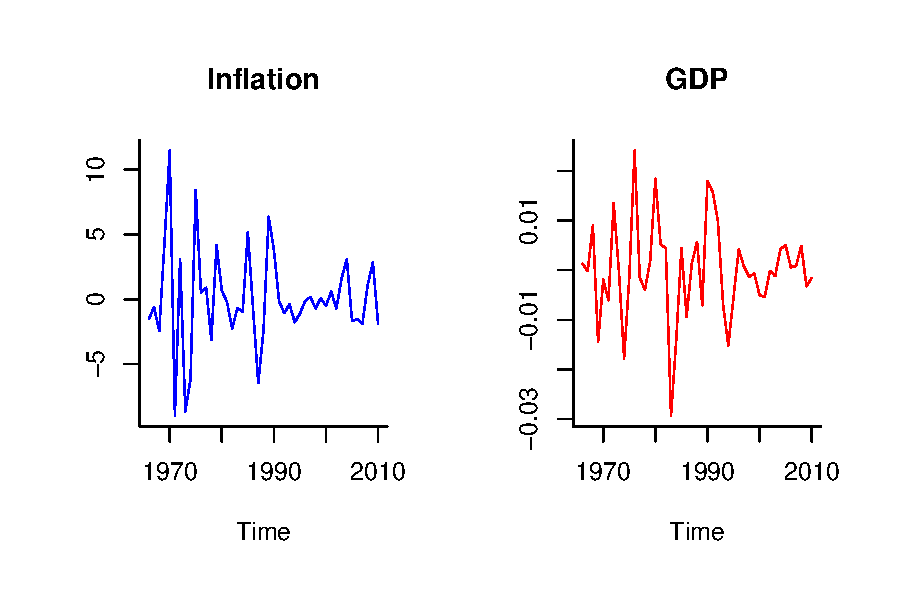
\includegraphics[scale=0.601]{inflation.eps} 
\end{figure}

When the cyclic components of money supply and inflation it appears that the cyclic component of inflation is characterized by a higher frequency of fluctuations than that of money supply. This in a way, suggest that inflation in Tanzania is not purely a monetary phenomenon; and that other real and structural factors influence the rate of inflation.

\subsubsection{Government Expenditure}

Figure 7 presents the estimate of the cyclic component of government expenditure, and also an estimate of the cyclic component of GDP for comparison.

\begin{figure}[ht]
\centering
\begin{small}
\caption{Cyclic Component of Government Expenditure}
\end{small}
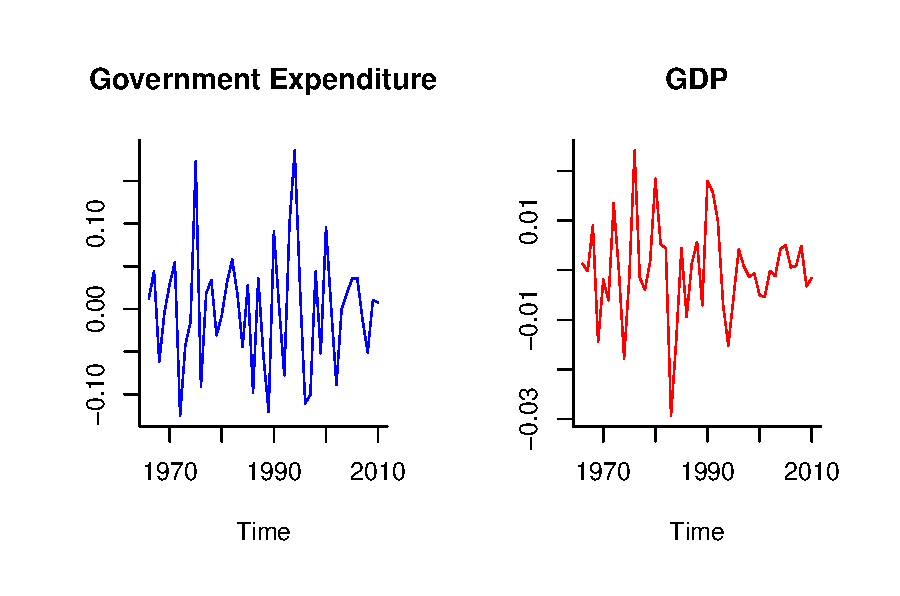
\includegraphics[scale=0.601]{gov_expend.eps} 
\end{figure}

More or less the cyclic component of government expenditure behaves like those of GDP, money supply, and inflation.  It is characterised by big fluctuations between 1996 and 1992, and relatively milder fluctuations after 1992. This in a way could be reflecting the government's commitment to a more stable fiscal policy in the post economic reform period.

\newpage
\subsection{Business Cycles and Tax Revenue}

In this section, estimates of business cycles for tax revenue are presented.  Cyclic components of total tax revenue, income tax, import and excise duties, and othe taxes (as a category) have been estimated for the period 1966 - 2013. It was not possible to estimate the cyclic components of more disaggregaed categories of taxes due to unavailability of data before 1998. In addition to presenting the esstimates of the cyclic componts of the tax revenue, the behaviour of these cyclic components is compared to the behaviour of the cyclic component of GDP.

\subsubsection{Total Tax Revenue}

The estimate of the cyclic component of total tax revenue is presented in Figure 8 (left panel). On the right panel, the estimate of the cyclic component of GDP (the major tax base) is presented for comparison.

\begin{figure}[ht]
\centering
\begin{small}
\caption{Cyclic Component of Tax Revnue}
\end{small}
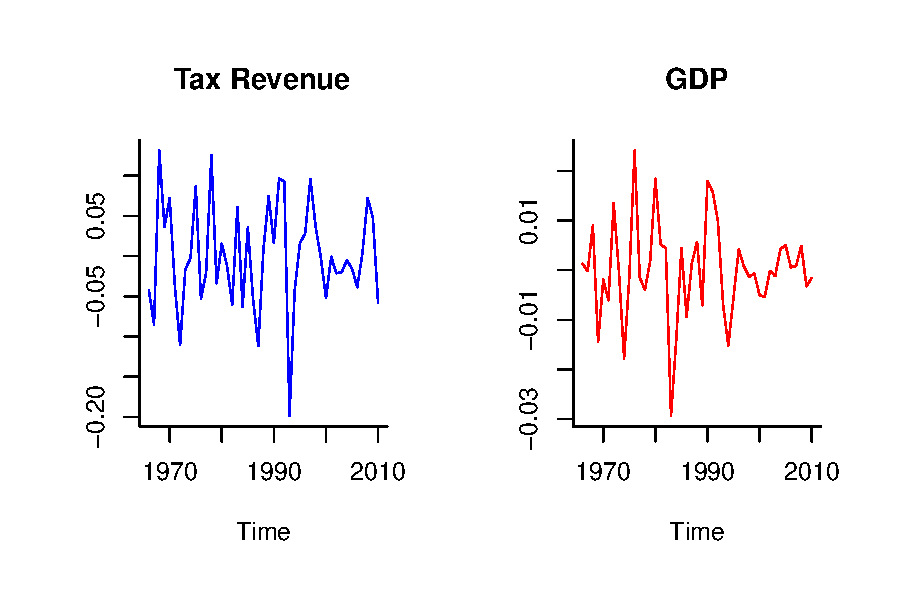
\includegraphics[scale=0.601]{tax_revenue.eps} 
\end{figure}

As it can be observed in the Figure, generally speaking, the cyclic component of total tax revenue behaves more or less like that of GDP.  First, just like in the case of GDP, the cyclic component of total tax revenue is characterized by 3 major cycles between 1966 and 1992, and relatively milder fluctuations thereafter. Second, the peaks and troughs of the two cyclic components are more or less synchronized. For example, both cyclic components are characterized by peaks roughly in 1967, 1976 and 1996.  Similarly, both components are charecterized by troughs roughly in 1970, 1983 and 1992.

\newpage
\subsubsection{Income Tax}

Figure 9 presents the estimate of the cyclic component of income tax together with the estimate of the cyclic component of GDP for comparison.

\begin{figure}[ht]
\centering
\begin{small}
\caption{Cyclic Component of Income Tax}
\end{small}
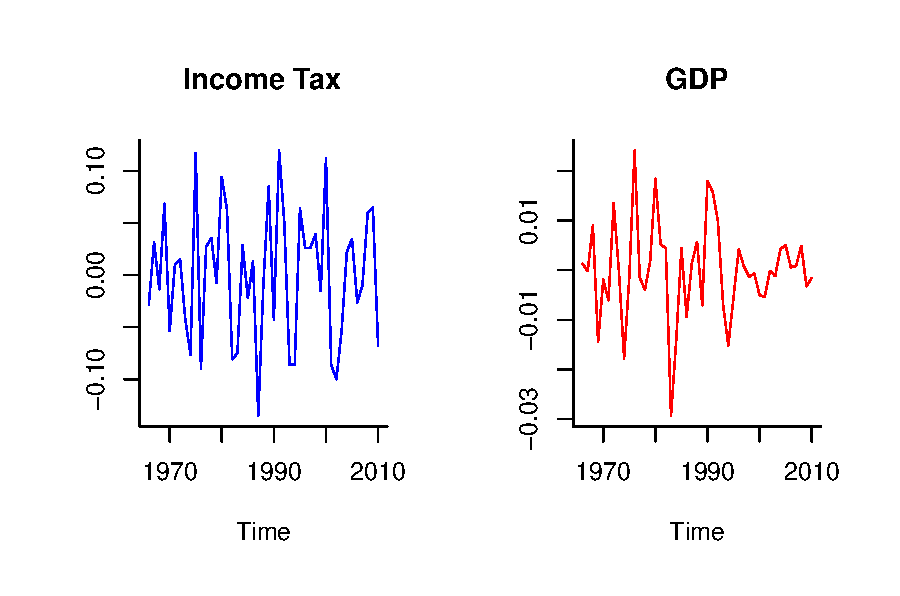
\includegraphics[scale=0.601]{income_tax.eps} 
\end{figure}

A closer observation of Figure 9 reveals that the cyclic component of income tax behave more less like that of total tax revenue.  This is not suprising because income tax is one of the components that make up the total tax revenue. Just like the cyclic component of total tax revenue, the cyclic component of income tax is characterized by 3 major cycles between 1966 and 1992, and a period of relatively mild fluctuations thereafter. The peaks and troughs of the cyclic component of income tax are sychronized with those of the cyclic component of GDP.

\subsubsection{Import and Excise Duties}

The estimate of the cyclic component of import and excise duties is presented in Figure 10. On the right panel of the same Figure, the cyclic component of GDP is also presented for comparison.

\begin{figure}[ht]
\centering
\begin{small}
\caption{Cyclic Component of Import and Excise Duties}
\end{small}
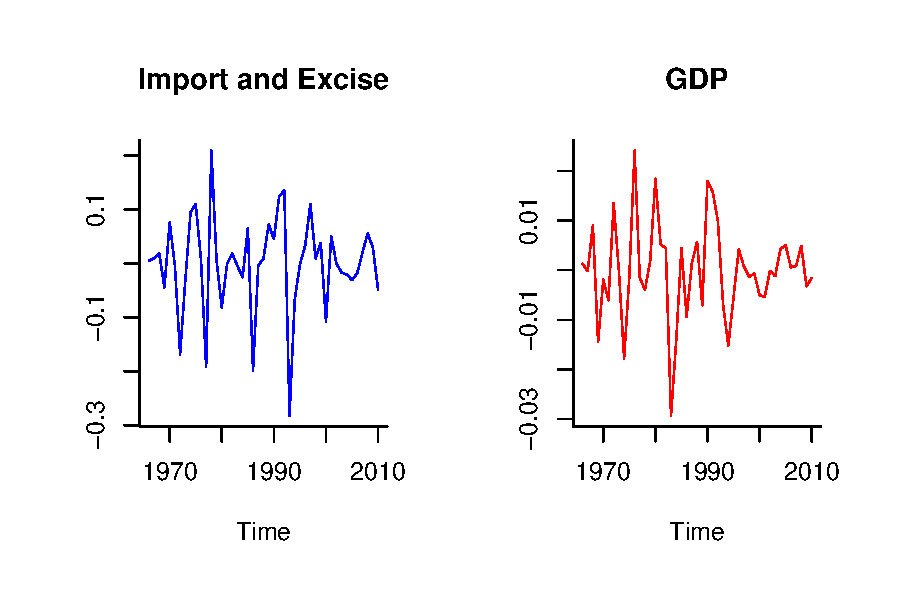
\includegraphics[scale=0.601]{import_taxes.eps} 
\end{figure}

The behavior of the cyclic component of import and excise duties is similar to those of total tax revenue, income tax and GDP. It is also characterized with 3 major cycles between 1966 and 1992, with the period after 1992 being characterized by relatively milder fluctuations.  The peaks and troughs of the cyclic component of import and excise duties are also more or less synchronized with those of GDP.

\subsubsection{Other Taxes}

Figure 11 presents the estimate of the cyclic component of other taxes. In the same Figure, the estimate of the cyclic component of GDP is also presented for comparison.

\begin{figure}[ht]
\centering
\begin{small}
\caption{Cyclic Component of Other Taxes}
\end{small}
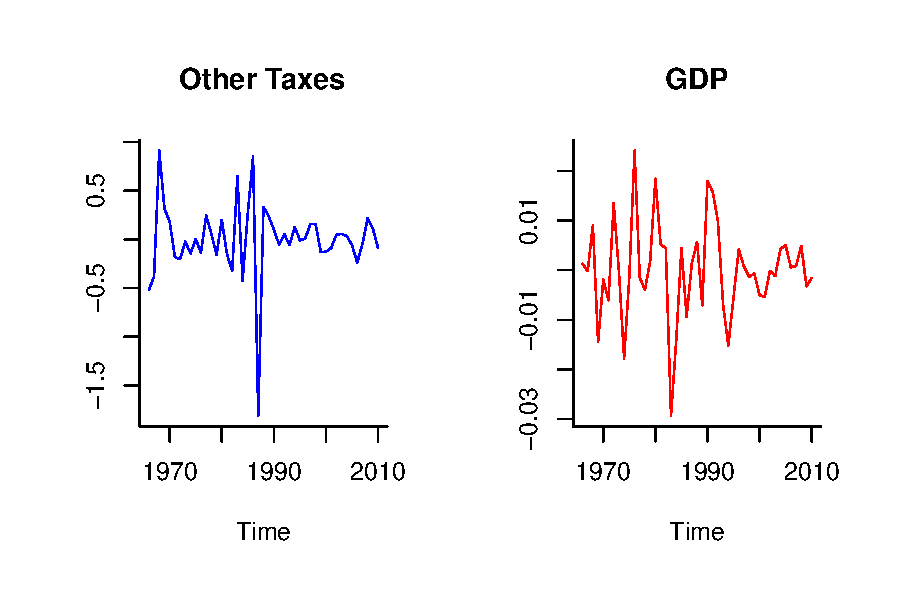
\includegraphics[scale=0.601]{other_taxes.eps} 
\end{figure}

It is interesting to note that the cyclic component of other taxes behave significantly differently from the cyclic components of GDP and those of other macroeconomic varaiables. For example, with the exception of the period roughly between 1982 and 1987, the fluctuations have been more or less mild for almost all the entire study period. 

Moreover, the peaks and troughs of the cyclic component of other taxes do not appear to be synchronized with those of GDP. For example, while for other taxes, the peaks are found roughly in 1970, 1983 and 1986, for GDP the peaks are found in 1967, 1976 and 1996. While for other taxes the troughs are found roughly in 1976, 1985 and 1988, for GDP the troughs are found roughly in 1970, 1983 and 1992.  It seems other taxes have been counter-cyclical. For example, while other taxes experienced a trough in 1976, GDP registered a peak. 

In summary, two points are noteworthy. First, it can be argued that during the study period, Tanzania experienced 3 major business cycles between 1966 and 1992, and relatively mild fluctutions thereafter. Second, with the exception of other taxes, the peaks and troughs in the other macroeconimc variables are synchronized with the peaks and troughs in GDP. This \textit{suggests} that, with the exception of other taxes, the other macroeconomic variables have been pro-cyclical.  To know whether exactly these variables have been pro-cyclical or not is an issue which will be addressed in the later sections.


\subsection{Seasonal Cycles and Tax Revenue by Disagreggated Sector}
In this Section, cyclic components of revenue from disaggregated sectors are estimated; and these componets are compared to sectoral GDP, which are the tax bases for respective taxes.  Use is made of the quartely data from the first quota of 2001 to the fourth quota of 2014. Given this short study  period in which a full cycle can be complete in a period less than a year, basically one can not call these estimates \textit{business cycles} \footnote{Acording to the common use of the terminology, a typical complete business cycle lasts for at least a year}. These estimates can rather be called \textit{seasonal fluctuations/cycles}.

\subsubsection{Agricuture}

The Figure below presents the cyclical component of tax revenue from the agricural sector and the cyclic component of the agricultural GDP.

\begin{figure}[ht]
\centering
\begin{small}
\caption{Cyclic Component of Tax Revenue from Agriculture}
\end{small}
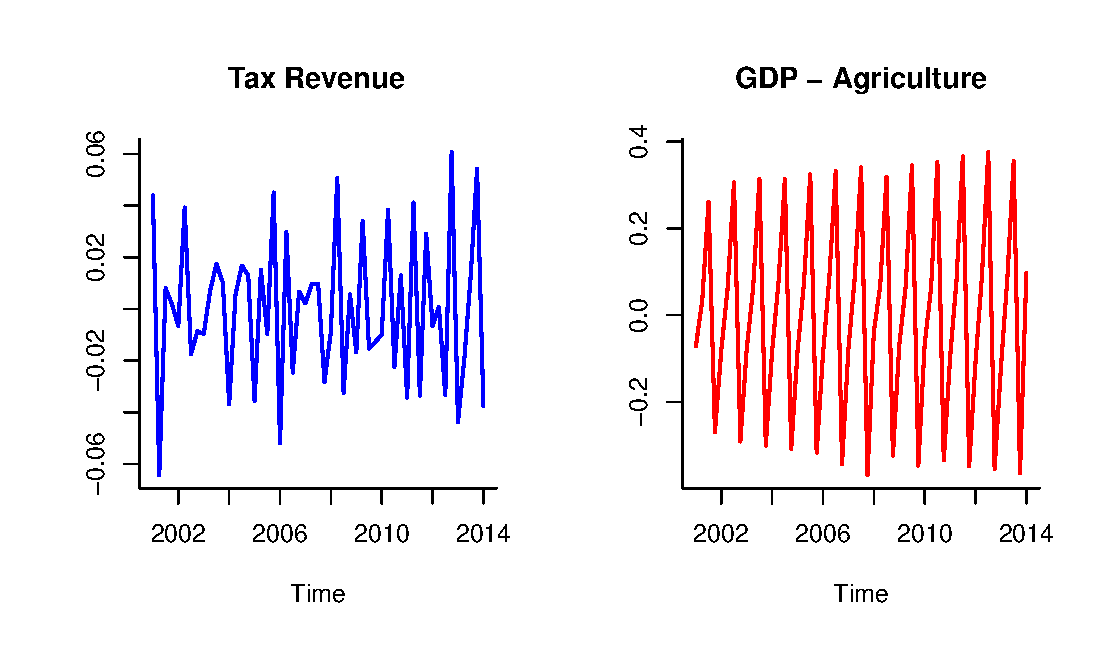
\includegraphics[scale=0.601]{agric.eps} 
\end{figure}

From the Figure, two major observations can be made. First, the cyclic estimate of the agricultural GDP seems to be more volatile than the estiate of the cyclic component of tax revenue from the agricultural sector. Second, the cyclic components are not syncronized.  As it can been observed from the Figure, when tax revenue from the agricultural sector records a peak, agricultural GDP records a trough, and vice versa.

This counter-cyclic behavior would seem to be contrary to \textit{`conventional wisdom'}, and also contrary to what has been observed for the aggregate variables (both in terms of sectoral and time aggregation).  A plausible explanation for this behavior is the fact that the aggregation conceals the actual behavior of the variables through the effects of averaging of the movements in the variables in the process of aggregation. In this case, the counter-cyclic behavior of the two variables can be explained by the fact that the sectorl output performance has a lagged impact on tax revenue. For example, a boom in the agriculture sector in the current quarter will lead to increased tax revenue in the next quarter.  

\subsubsection{Mining}

The estimates of the cyclical components of tax revenue from the mining sector and mining GDP are shown in the Figure 13 below. Unlike in what has been observed in the preceding section in the case of the agriculture, the cyclic components of revenue from the mining sector and the cyclic component of mining GDP are syncronized.

\begin{figure}[h]
\centering
\begin{small}
\caption{Cyclic Component of Tax Revenue from Mining}
\end{small}
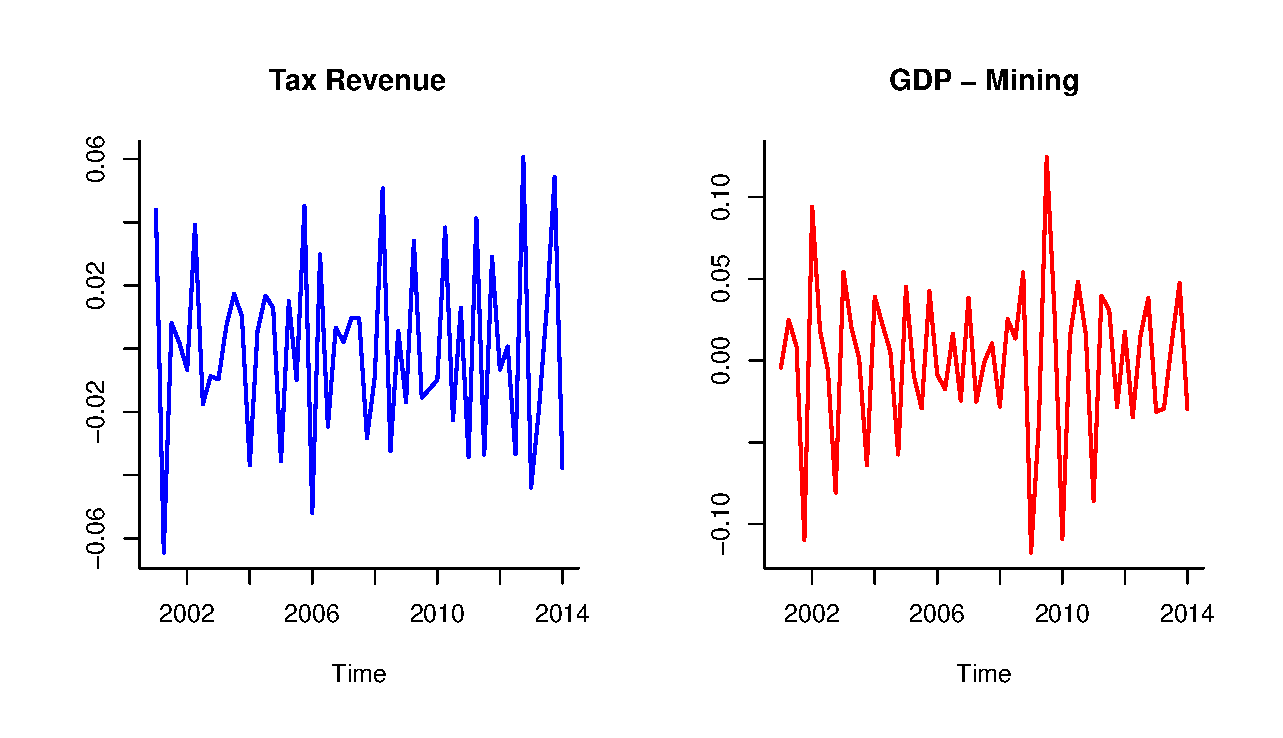
\includegraphics[scale=0.601]{mining.eps} 
\end{figure}

As it can be observed from the Figure, peaks and troughs in the two variables occur simultaneously across the cycle, suggesting that revenue from the mining sector is pro-cyclic.


%\newpage

\subsubsection{Manufacturing}

One of the sectors that over the past decade have recorded high growth rate in tax revenue generation is manufacturing.  Figure 14 below presents the estimates of the cyclic component of tax revenue from the manufacturing sector together with the estimate of the cyclic component of manufacturing GDP.


\begin{figure}[h]
\centering
\begin{small}
\caption{Cyclic Component of Tax Revenue from Manufacturing}
\end{small}
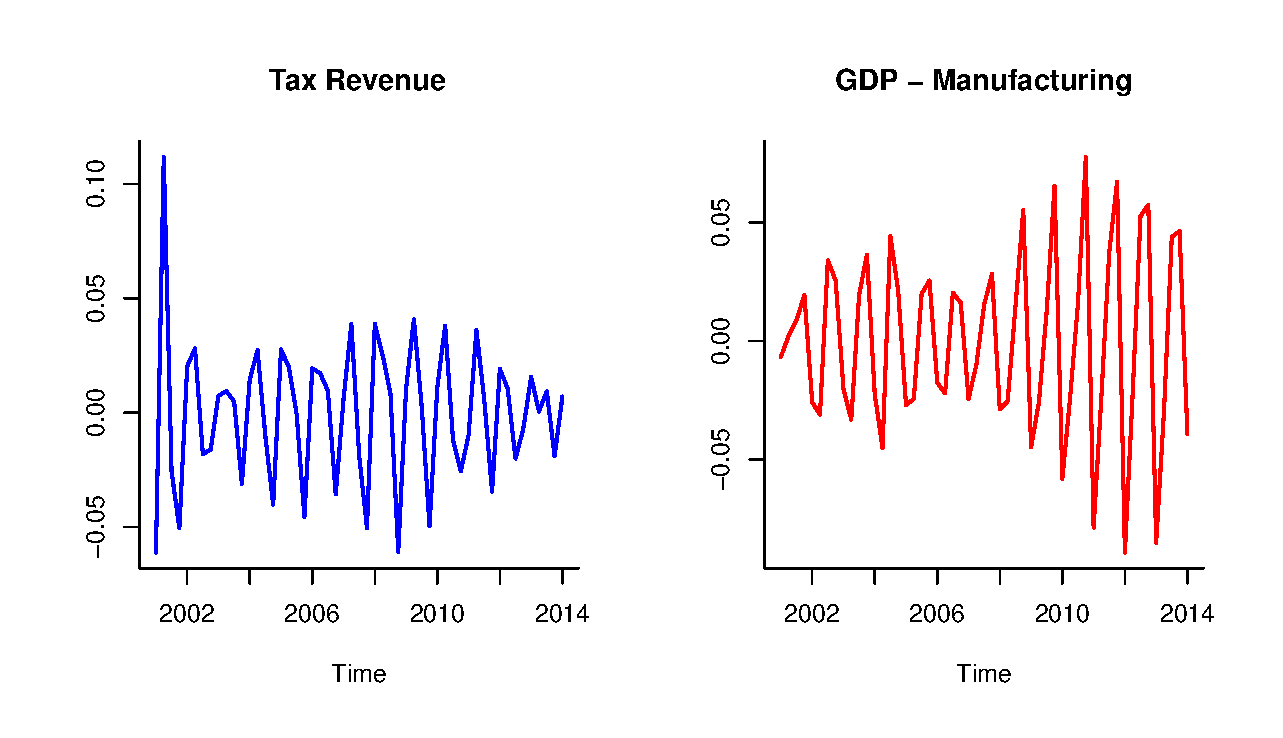
\includegraphics[scale=0.601]{manufac.eps} 
\end{figure}

Two major observations can be made from the Figure. First, while high volatility characterized the early study period in the case of revenue from the manufacturing sector, high volatility characterized the late period of the study in the case of manufacturing GDP. Secondly, just like in the case of the agriculture sector, the peaks and troughs of manufacturing tax revenue and manufacturing GDP are not synchronized.

%\newpage
\subsubsection{Electricity}

Electricity is the sector one of the top two sectors that recorded high growth rate (5.9 percent) between 2001 and 2014. The estimates of the cyclic components of the sector's revenue generation and GDP are presented in Figure 15.


\begin{figure}[h]
\centering
\begin{small}
\caption{Cyclic Component of Tax Revenue from Electricity}
\end{small}
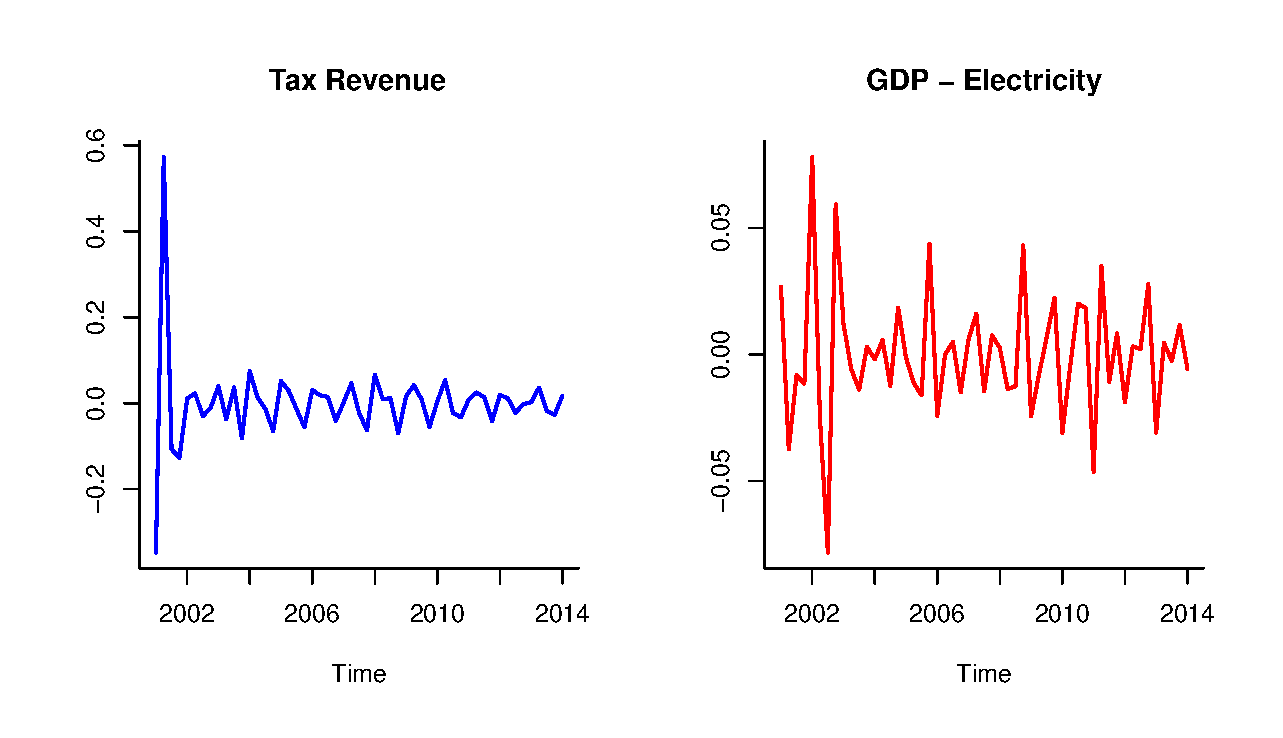
\includegraphics[scale=0.601]{electric.eps} 
\end{figure}

One can observe two noteworthy points from the Figure. First, with the exception of the first three quarters of the 2001 - 2014 period, volatility of of tax revenue from electricity sector was fairly low compared to that of the sector's GDP. Second,the peak and troughs for the sector's revenue and GDP are not syncronized, just like in the case of agriculture and manufacturing sectors.


\subsubsection{Construction}

Figure 16 presents the estimates of the estimates of the cyclic components of both revenue from the construction sector and construction GDP.

\begin{figure}[h]
\centering
\begin{small}
\caption{Cyclic Component of Tax Revenue from Contruction}
\end{small}
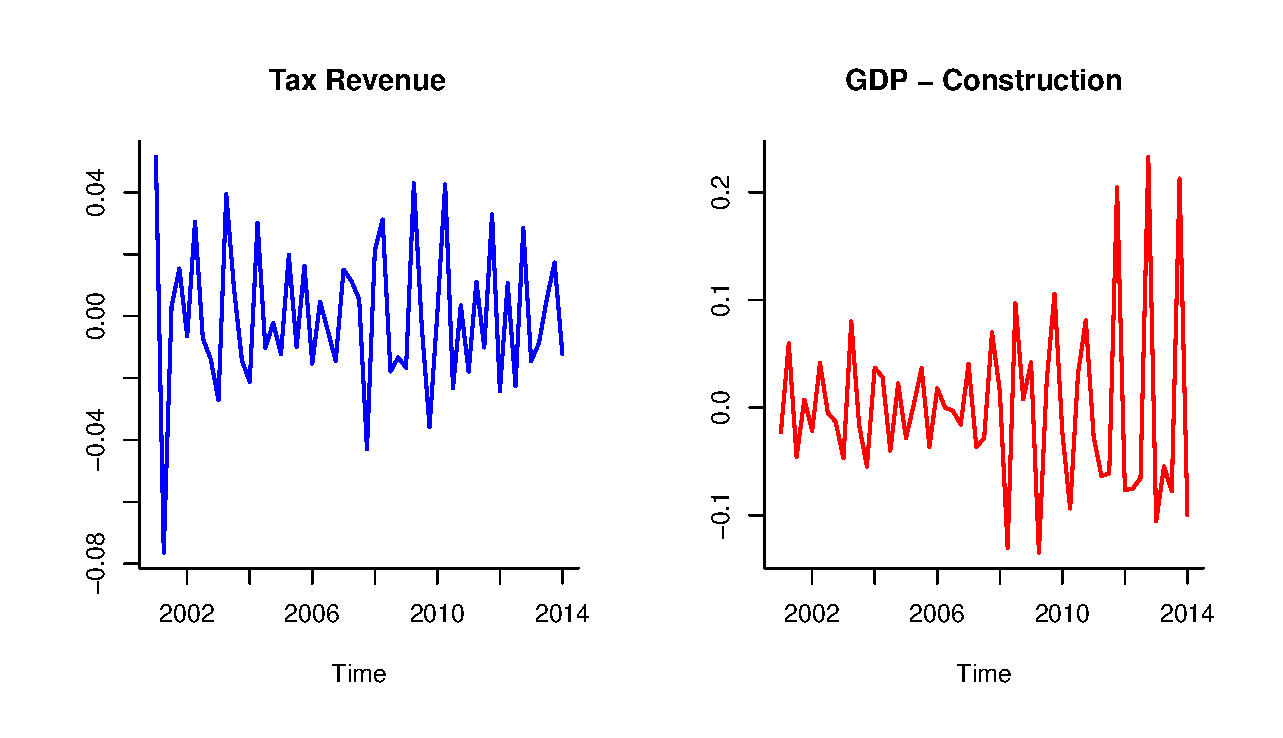
\includegraphics[scale=0.601]{construct.eps} 
\end{figure}

It is clear from the Figure that construction GDP has been relatively more volatile that tax revenue from the construction sector, particularlry during the end of the 2001 - 2014 period.

\subsubsection{Trade}

Trade in this context is defined to include wholesale and retail trade, repair of motor vehicles and motorcycles. The estimates of the cyclic components of the sector's revenue generation and GDP are presented in Table 17. 

\begin{figure}[h]
\centering
\begin{small}
\caption{Cyclic Component of Tax Revenue from Trade}
\end{small}
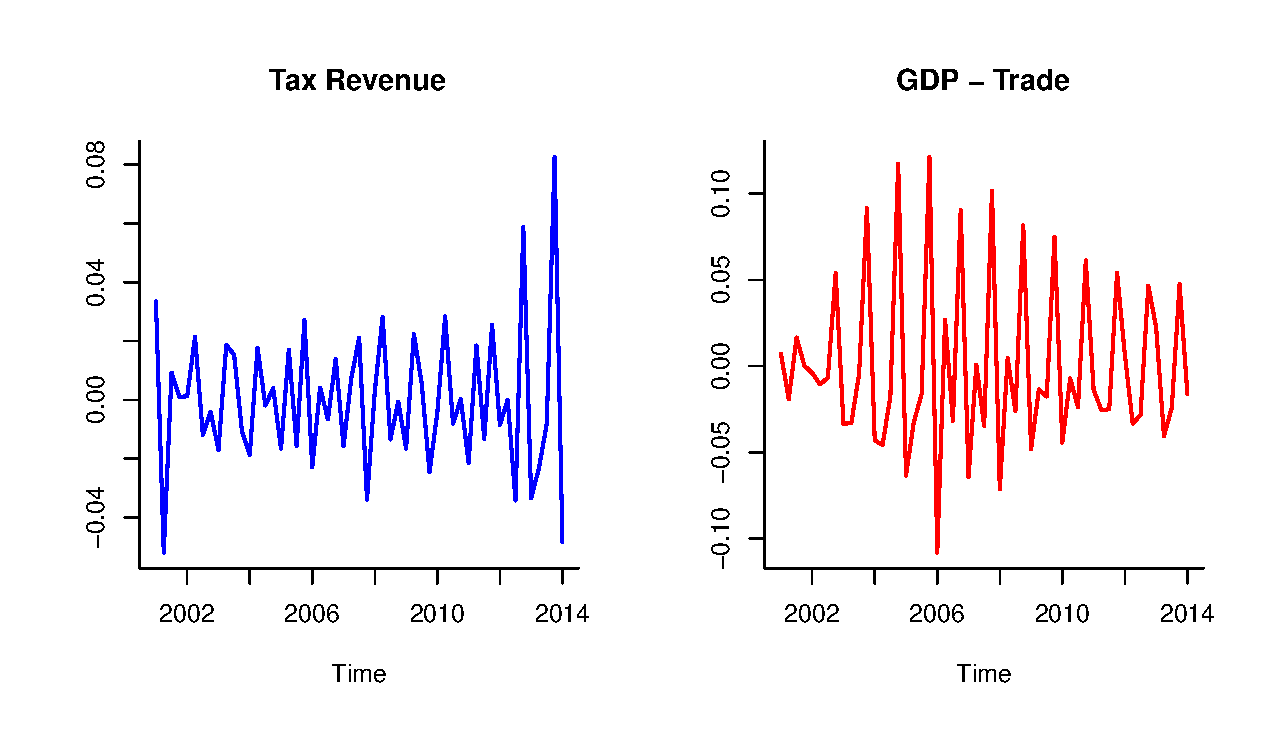
\includegraphics[scale=0.501]{trade.eps} 
\end{figure}

The Figure reveals two important matters. First, the peaks and troughs for sector's tax revenue and GDP are not synchronized. Second,the sector's GDP has been more volatile than the sector's tax revenue generation.

\subsubsection{Transport}

Transport in this study is defined to include transportation and storage. This is one of the sectors that has been growing fast. Over the 2001 - 2014 period, the average growth rate is estimated to have been 5 percent.  Figure 18 presents the estimates of the cyclic components of tax revenue and GDP for the sector.


\begin{figure}[h]
\centering
\begin{small}
\caption{Cyclic Component of Tax Revenue from Transport}
\end{small}
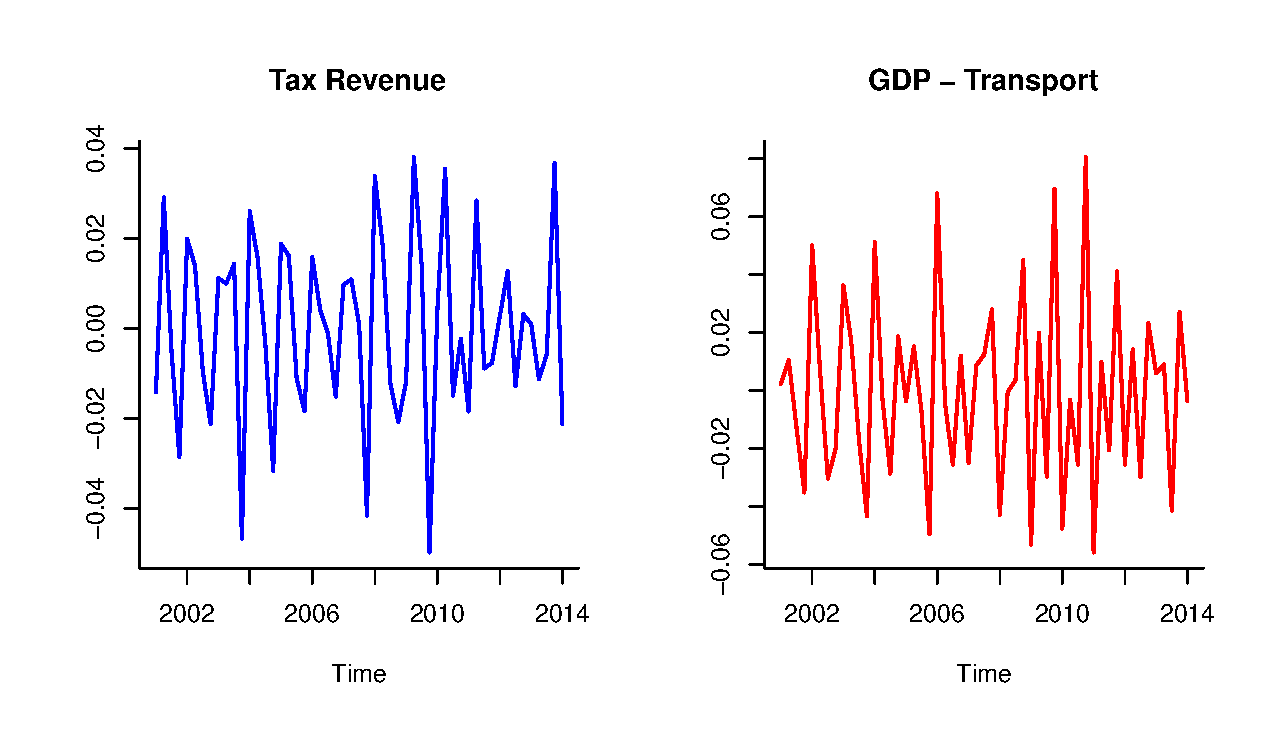
\includegraphics[scale=0.501]{transport.eps} 
\end{figure}

Two important points emerge upon closely examining the Figure. First, the sector's GDP has relatively been more volatile than the sector's revenue generation. Second, the peaks and troughs for the sector's tax revenue generation and GDP seem to be more or less synchronized.


\subsubsection{Financial Services}

In this study, financial services are defined to include financial and insurance activities.  The estimates for the cyclical components of tax revenue generation and GDP for the sector are shown in the Figure below.

\begin{figure}[h]
\centering
\begin{small}
\caption{Cyclic Component of Tax Revenue from Financial Services}
\end{small}
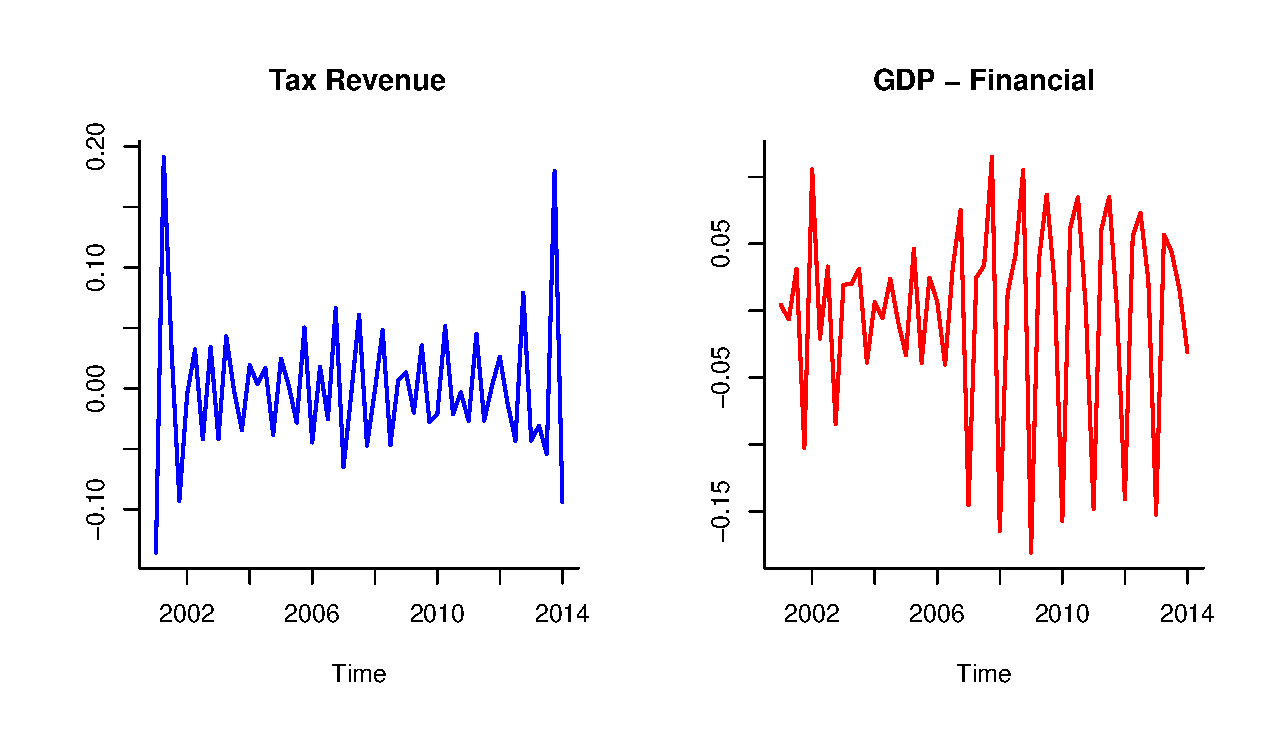
\includegraphics[scale=0.501]{financial.eps} 
\end{figure}

Upon close examination of the Figure, two major issues can be noted.  First, thhe sector's GDP has been relatively more volatile the the sector's tax revenue generation. Second, the peaks and troughs in the cyclic components of tax revenue generation and GDP for the sector appear to be synchronized.


\subsubsection{Real Estates}

Estimates of the cyclic components of tax revenue and GDP for the real estates sector is presented in Figure 20 below. A close examination of the Figure reveals that the behavior of this sector more or less similar to the behavior of most of the sectors that have been examined in this section.

\begin{figure}[h]
\centering
\begin{small}
\caption{Cyclic Component of Tax Revenue from Real Estates}
\end{small}
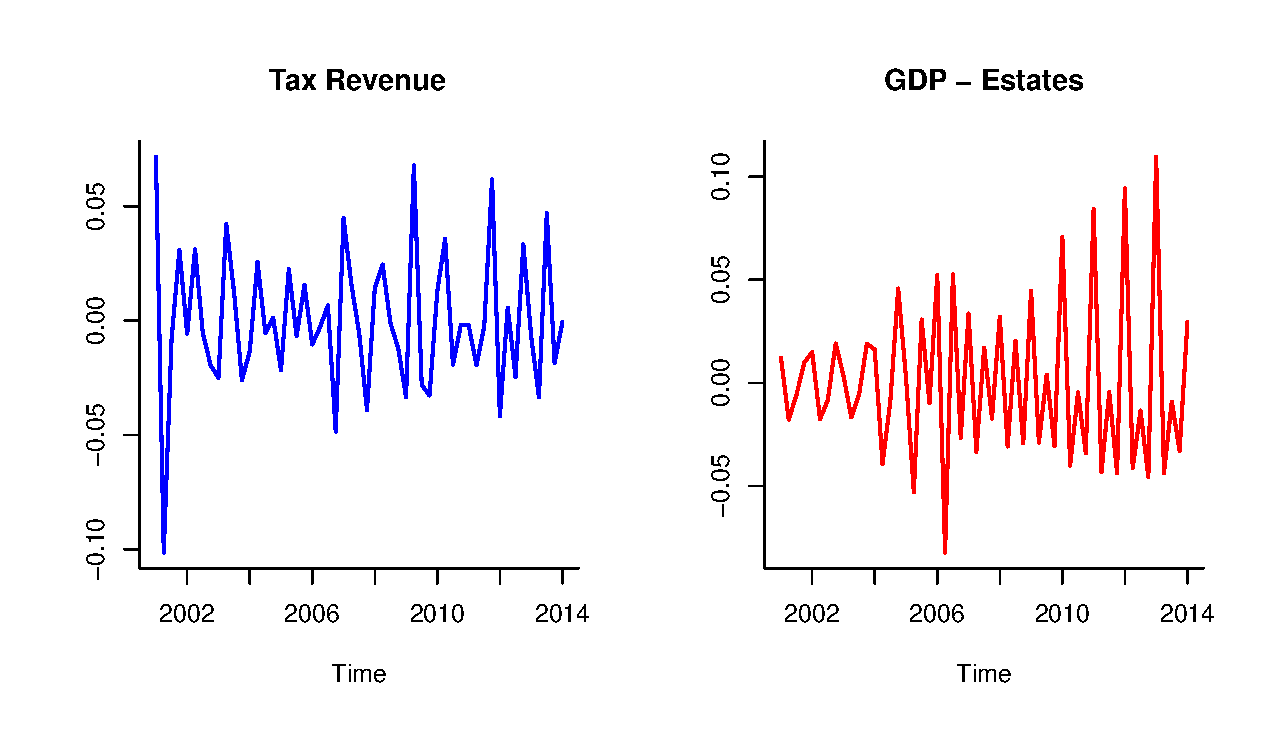
\includegraphics[scale=0.501]{estates.eps} 
\end{figure}

The sector's GDP has been relatively more volatile than the sector's tax revenue generation. Inaddition, the peaks and troughs of tax revenue generation and GDP for the sector are synchronized.

%\newpage
In summary, as far as estimation of the cyclical components of sectoral tax revenue and GDP using quarterly data for the period 2001 - 2014, two major points can be noted. First, unlike in the case of annual data for the period 1966 - 2010, for quartely data for the period 2001 - 2014, results indicate that with the exception of mining, trade, transport and financial services sectors the output fluctuations are counter-cyclical, contrary to the \textit{`stylized facts'}. 

In thses cases, peaks and troughs of sectoral tax revenue generation are not synchronized with those of sectoral GDP. The plausible explanation here is that the sectoral output performance is translated into tax revenue prformance affter a time lag. This behavior is concealed in the annual data due to the effect of avraging out in the process of time aggregation in the case of time series data. Second for most of the sectors, GDP appears to be more volatile than tax revenue generation.
%\newpage
\subsection{Are the Variables Pro-cyclical or Counter-cyclical?}

\subsubsection{Business Cycles}

A variable is said to be \textit{pro-cyclical} when it experiences boom (recession) as GDP experiences a boom (recession); and it is said to be \textit{counter-cyclical} when it experiences a boom (recession) as GDP experiences a recession (boom). In this section, simple correlation coeffients between the cyclic component of a macroeconomic variable and a cyclic component of GDP, which are usually used to determine whether a variable is pro-cyclical or counter-cyclical are presented.  Table \ref{tab2} below presents the Kendall's correlation coefficients between the cyclic components of individual macroeconomic variables and a cyclic component of GDP.


\begin{table}[h]
\centering
\begin{small} 
\caption{Kendall's Correlation Coefficients} 
\label{tab2}
\begin{tabular}{l c }
\toprule
\multicolumn{1}{l}{\textbf{Variable}} & \textbf{Coefficient}\\ 
 \midrule
Total tax revenue & 0.069 \\
Income tax & 0.053 \\
Import and excise duties & 0.137\\
Other taxes  & -0.061\\
Money supply (M2) & 0.071 \\
Inflation & 0.065\\
\bottomrule
\end{tabular}
\end{small}
\end{table}
 

In general the findings appear to confirm what was presumed in the previous section. With the exception of other taxes, the correlation coefficients for all macroeconomic variables are positive, indicating that these variables are pro-cyclic. That is when GDP is in a boom, they are also in a boom; and when GDP is in recession, they are also in recession. 

In the case of tax revenue, this is the expected behaviour. One would expect to collect more tax revenue when the tax base expand, and collect less when the tax base shrinks. In this case, the behavior of income tax and import and excise duties appear to be consistent with the \textit{conventional wisdom}; and the behaviour of other taxes appears to be contrary to the \textit{conventional wisdom}.

\subsubsection{Seasonal Cycles}

In this section the focus is on examining  whether the sectoral tax revenue seasonal cycles are pro-cyclic or counter-cyclic. Table \ref{tab3} below presents  the Kendall's correlation coefficients between the cyclic components of tax revenue and GDP for the sectors.

\begin{table}[h]
\centering
\begin{small} 
\caption{Kendall's Correlation Coefficients} 
\label{tab3}
\begin{tabular}{l c}
\toprule
\multicolumn{1}{l}{\textbf{Sector}} & \textbf{Coefficient}\\ 
 \midrule
Agriculture & -0.292 \\
Mining & 0.053 \\
Manufacturing & -0.448\\
Electricity  & -0.163\\
Construction & -0.013 \\
Trade & 0.190\\
Transport & 0.176\\
Hotels & -0.064\\
Financial services & 0.042\\
Real estates & -0.09\\
Education & -0.292\\
Health & -0.055\\
\bottomrule
\end{tabular}
\end{small}
\end{table}

The Table reveals that, with the exception of mining, trade, transport, and financial services, tax revenue for the sectors is counter-cyclical (in the context of seasonal fluctuations).  This behavior can be explained by the fact that changes in economic activities in the sector affects tax revenue generation after a time lag. That is, an increase/decrease in the economic activity in the current quarter will lead to an increase/decrease in tax revenue in the next quarter.

\subsection{Volatility}

\subsubsection{Business Cycles}

The other interesting aspect in business cycle studies is the volatility of business cycles. Volatility as a concept tells something about the magnitude of downward and upward swings of the business cycles. Variance or standard deviation of the cyclic component is commonly used to measure volatility of business cycles. Usually a relatively large value of the variance or standard deviation will indicate, and a relatively low value of variance or standard deviation will indicate low volatility of business cycles. Table \ref{tab4} below presents standard deviations of the cyclic components of GDP and other macroeconomic variables.

\begin{table}[h]
\centering
\begin{small} 
\caption{Volatility Measures of Cyclic Components} 
\label{tab4}
\begin{tabular}{l c}
\toprule
\multicolumn{1}{l}{\textbf{Variable}} & \textbf{(Std. deviation)}\\ 
 \midrule
GDP & 0.0098\\ 
Total tax revenue & 0.067 \\
Income tax & 0.064 \\
Import and excise duties & 0.090\\
Other taxes  & 0.40\\
Money supply (M2) & 0.051 \\
Inflation & 3.81\\
\bottomrule
\end{tabular}
\end{small}
\end{table}

While fluctuations in inflation appear to be the most volatile, fluctuations in GDP are the least volatile.  For tax revenue, fluctuations in other taxes are the most volatile, and fluctuations in income tax are the least volatile. 

\newpage
\subsubsection{Seasonal Cycles}

This section presents the measures of seasonal fluctuations volatility in Table \ref{tab5} below.  With the exception of electricity, education and health, GDP fluctuations are more volatile than the flucuations of tax revenue. 

\begin{table}[h]
\centering
\begin{small} 
\caption{Volatility Measures (Standard Deviation) by Sector} 
\label{tab5}
\begin{tabular}{l c c}
\toprule
\multicolumn{1}{l}{\textbf{Sector}} & \textbf{Tax revenue} & \textbf{GDP}\\ 
 \midrule
Agriculture & 0.029 & 0.241\\
Mining & 0.029 & 0.048\\
Manufacturing & 0.031 & 0.039\\
Electricity  & 0.102 & 0.026\\
Construction & 0.024 & 0.077 \\
Trade & 0.024 & 0.050\\
Transport & 0.021 & 0.033\\
Hotels & 0.027 & 0.050\\
Financial services & 0.057 & 0.075\\
Real estates & 0.031 & 0.039\\
Education & 0.023 & 0.017\\
Health & 0.032 & 0.002\\
\bottomrule
\end{tabular}
\end{small}
\end{table}

With the exception of the financial services sector, which is characterized by relatively high volatility in both tax revenue and GDP, there seems to be no systematic relationship volatility in tax revenue and GDP. For example, the agricultural sector which is characterized by high volatility in GDP, its tax revenue volatility is relatively low. Regarding GDP, the agriculture sector is characterzed by relatively high volatility, and health sector is characterized by low volatility.  As for tax revenue, volatility is high in the electricity sector, and relatively low in the transport sector.

\subsection{Sources of Business Cycles in Tanzania}

In this section, factors that drive the business cycles in Tanzania are examined. A simple vector autoregressive model presented in Section 2.4.1 has been used to carry out the analysis. Granger - causality test and variance decomposition have been used to determine whether it is monetary factor or real factors wnich influence business cycles/macroeconomic fluctuations in Tanzania. Table \ref{tabvar} presents below the Granger - causality test statistics.

\begin{table}[h]
\centering
\begin{small} 
\caption{Granger - Causality Test} 
\label{tabvar}
\begin{tabular}{l c c}
\toprule
\multicolumn{1}{l}{\textbf{Null hypothesis}} & \textbf{Test statistic} & \textbf{P -- Value}\\ 
 \midrule
Money supply (M2) does not Granger-cause GDP  & 12.643 & 0.00064\\
GDP does not Granger-cause  M2 & 0.029 & 0.8362\\
There is no instant causality between M2 and GDP & 3.4225 & 0.0643\\
\bottomrule
\end{tabular}
\end{small}
\end{table}

The Table reveals that while it is possible reject the null hypothesis at 1 percent significance level, and conclude that money Granger -- causes GDP; it is not possible to reject the null that GDP does Granger - cause money supply at all conventional significance levels. Variance decomposition results appear to be consistent with the Granger - causality test results. Over the 10 -- period forcasting horizon, about 25 percent of the variations in GDP are caused by shocks in money supply, 75 percent of the variations in GDP are caused by shocks in GDP itself. 

In this case, variations in GDP due to shocks in GDP itself can be considered to be the shocks originating from random variations in real factors.  Thus, it can be said that \textit{both real and monetary factors are the causes of business cycles in Tanzania}; and also it can be said that  \textit{about 75 percent of the business cycles are due to real factors and 25 percent are due to monetary factors}. 

\subsection{Long Term Movements in Tax Revenue and Tax Bases}

This section examines the relationship between long term movemens in tax bases and long term movements in tax revenue.  The main issue which is addressed is: Does long term trends in tax revenue respond to long term trends in tax revenue. More specicically, this section examines whether tax revenue and tax bases are cointegrated, that is whether they have long run equlibrium relationship.  Unfortunately, the time period  of time series of tax revenue and GDP by sectors is too short (14 years) to give reliable cointegration test results\footnote{At least 30 annual observations are required for reliable cointegration test results.}. 

\begin{figure}[h]
\centering
\begin{small}
\caption{Trends of Import Duty, Income Tax and GDP}
\label{fig_grev}
\end{small}
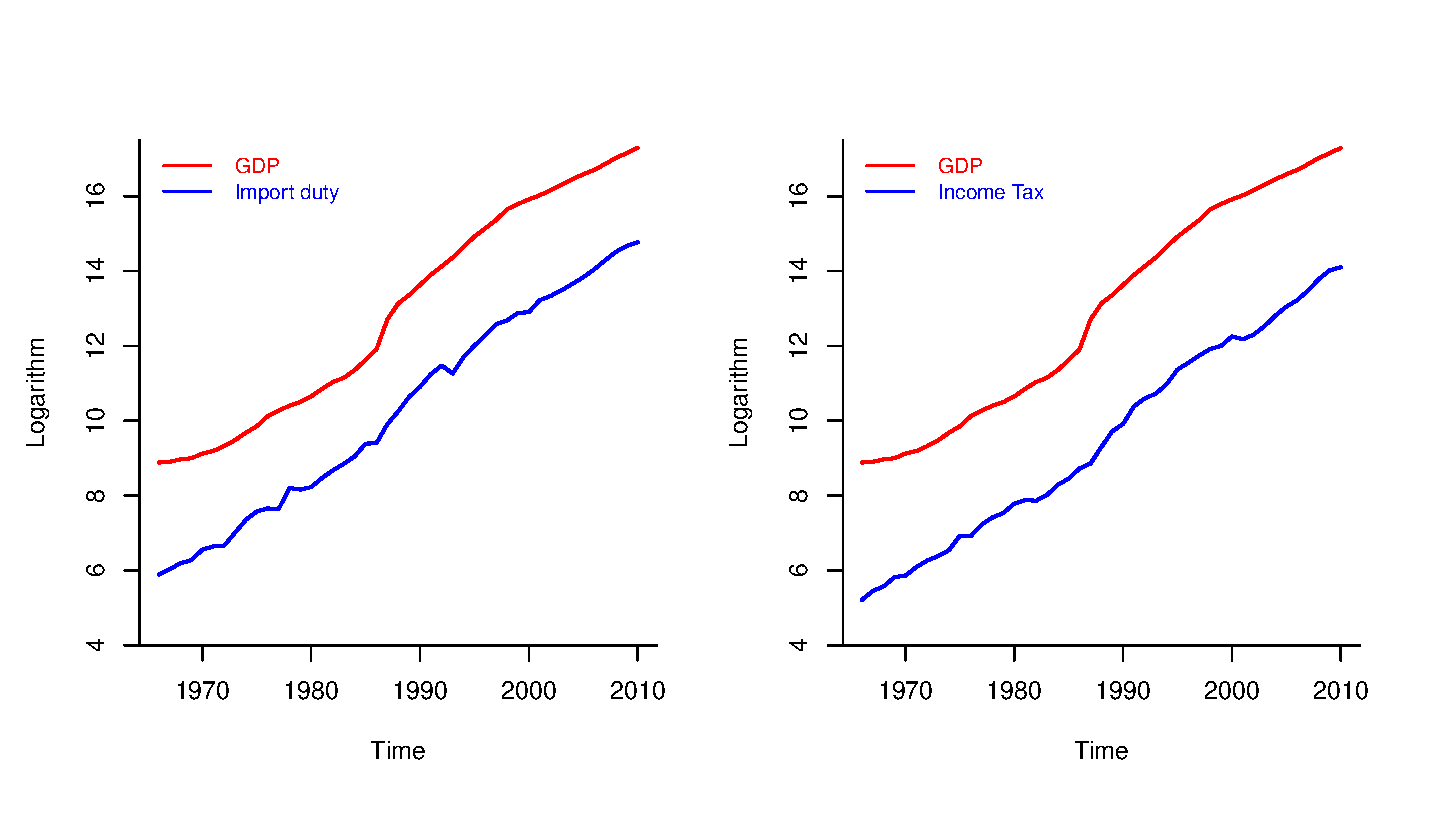
\includegraphics[scale=0.501]{taxi.eps} 
\end{figure}

\newpage
Fairly consistent and long time series are avaible for import duty, income tax and GDP for the period 1966 - 2010.  A close examination of Figure \ref{fig_grev} below suggests that long term trends for import duty and income tax have been moving together with the long term trend of GDP, without drifting apart over time.

The Figure suggests that long term trends in import duty and income tax have been responding to long term trend in GDP (the tax base). Inspite of a short period of 14 years for which the data is available,  a Phillips and Ouliaris contegration test has been carried out to examine if there is lon-run equilibrium relationship between sectoral tax revenue and sectoral GDP. The restults are reported in Table \ref{tabcoint} below.

\begin{table}[h]
\centering
\begin{small} 
\caption{Phillips -- Ouliaris Cointegration Test Results} 
\label{tabcoint}
\begin{tabular}{l c}
\toprule
\multicolumn{1}{l}{\textbf{Sector}} & \textbf{Test statistic}\\ 
 \midrule
Agriculture & 8.7922 \\
Mining & 1.1832 \\
Manufacturing & 1.5535\\
Electricity  & 22.0073\\
Construction & 3.8091 \\
Trade & 1.2755\\
Transport & 0.6798\\
Hotels & 0.9656\\
Financial services & 5.9030\\
Real estates & 3.7176\\
Education & 0.4705\\
Health & 1.4897\\
\bottomrule
\end{tabular}
\end{small}
\end{table}

The results suggest that there is no cointegration between sectoral tax revenue and sectoral GDP.  However, as it has been argued before these results are not reliable, because 14 years is too short a period for reliably examining long-run equilibrium relationship between variables.

\subsection{Link Between Business/Seasonal Cycles and Tax Revenue}
In this section a link between business/seasonal cycles and tax revenue by sector in examine. Results of estimation of a simple econometric model specified in the methodology section are presented. These results are tax elasticies.  The tax elasticity indicates the perentage by which tax revenue will increase/decrease as a result of 1 percentage increase in the tax base.  Table \ref{tab6} below presents the tax elasticities by sectors. Regression results for the estimates of elasticities are presnted in Tables \ref{tab8} - \ref{tab11} in the Appendix.

\begin{table}[h]
\centering
\begin{small} 
\caption{Tax Elasticities by Sectors} 
\label{tab6}
\begin{tabular}{l c}
\toprule
\multicolumn{1}{l}{\textbf{Variable}} & \textbf{Elasticity estimate}\\ 
 \midrule
Agriculture & 0.4 \\
Mining & 2.2 \\
Manufacturing & 2.3\\
Electricity  & 3.6\\
Construction & 1.5 \\
Trade & 2.0\\
Transport & 1.9\\
Hotels & 3.8\\
Financial services & 2.3\\
Real estates & 1.9\\
Education & 3.2\\
Health & 2.6\\
\bottomrule
\end{tabular}
\end{small}
\end{table}

With the exception of the agriculture sector, taxes are elastic and statistically significant at 1 percent of significance level. For these sectors, changes in the sectoral output are associated with more than proprtionate change in the tax revenue generated by the sector. 

\newpage
In the case of agriculture, the tax elasticity is not statistically different from zero even at 10 percent of significance level. This implies that tax revenue generated by the agriculture sector do not respond at all to changes in agricultural GDP. To some extent this can be explained by the fact that most of the activities in the sector are informal and are not captured by the tax net.


\section{Conclusion}

The main objective of this study has been to estimate the business cycles, and to examine the link between the business cycles and tax revenue performance. The outcome of this study is important in the sense of enabling TRA to monitor and track the developments in the macroeconomic variables, and thus be able to cushion tax revenues from the adverse effects of swings in the economic activity. The main findings of the study are as follows:

\subsection{Business Cycles}
\begin{compactenum}[(i)]
\item Over the study period, Tanzania experienced 3 major business cycles between 1966 and 1992, and relatively mild fluctutions thereafter,
\item  With the exception of other taxes, the peaks and troughs in the other macroeconimc variables (including income tax and import and excise duties) are synchronized with the peaks and troughs in GDP. the peaks are found in 1967, 1976 and 1996; and the troughs roughly in 1970, 1983 and 1992.
\item  With the exception of other taxes, the correlation coefficients for all macroeconomic variables are positive, indicating that these variables are pro-cyclic,
\item In the case of tax revenue, this is the expected behaviour. One would expect to collect more tax revenue when the tax base expand, and collect less when the tax base shrinks. In this case, the behavior of income tax and import and excise duties appear to be consistent with the \textit{conventional wisdom}; and the behaviour of other taxes appears to be contrary to the \textit{conventional wisdom}.
\item While fluctuations in inflation appear to be the most volatile, fluctuations in GDP are the least volatile.  For tax revenue, fluctuations in other taxes are the most volatile, and fluctuations in income tax are the least volatile. 
\end{compactenum}

\subsection{Seasonal Cycles}
\begin{compactenum}[(i)]
\item With the exception of mining, trade, transport, and financial services, tax revenue for the sectors is counter-cyclical (in the context of seasonal fluctuations).  This behavior can be explained by the fact that changes in economic activities in the sector affect tax revenue generation after a time lag. That is, increase/decrease in the economic activity in the current quarter will lead to an increase/decrease in tax revenue in the next quarter.
\item  With the exception of electricity, education and health, GDP fluctuations are more volatile than the flucuations of tax revenue. 
\item Tax revenue is elastic for almost all the sectors. Increase in sectoral GDP appears to lead to more than proportional changes in tax revenue generated by sectors. For the agricultural sector, tax revenue do not seem to respond to agricultural GDP.
\end{compactenum}

\newpage
\appendix
\section{Estimates of Growth Rates by OLS}

\begin{table}[bh]
\caption{Estimates of Growth Rates by OLS}
\label{tab7}
\begin{center}
\begin{tabular}{l D{.}{.}{2.7} D{.}{.}{2.7} D{.}{.}{2.7} }
\toprule
 & \multicolumn{1}{c}{Agriculture} & \multicolumn{1}{c}{Industry} & \multicolumn{1}{c}{Services} \\
\midrule
Intercept  & 6.9227^{***} & 9.9376^{***} & 10.9217^{***} \\
           & (0.0655)     & (0.0448)     & (0.0522)      \\
Time       & 0.0322^{***} & 0.0476^{***} & 0.0457^{***}  \\
           & (0.0017)     & (0.0011)     & (0.0013)      \\
\midrule
R$^2$      & 0.8520       & 0.9642       & 0.9483        \\
Adj. R$^2$ & 0.8498       & 0.9637       & 0.9475        \\
Num. obs.  & 68           & 68           & 68            \\
RMSE       & 0.2671       & 0.1827       & 0.2127        \\
\bottomrule
\multicolumn{4}{l}{\scriptsize{$^{***}p<0.001$, $^{**}p<0.01$, $^*p<0.05$}}
\end{tabular}
\end{center}
\end{table}

\section{Estimates of Tax Elasticities}
\begin{table}[bh]
\caption{Estimates of Tax Elasticities by OLS}
\begin{center}
\begin{tabular}{l D{.}{.}{2.5} D{.}{.}{3.7} D{.}{.}{3.7} }
\toprule
 & \multicolumn{1}{c}{Agriculture} & \multicolumn{1}{c}{Mining} & \multicolumn{1}{c}{Manufacturing} \\
\midrule
Intercept         & 3.0561   & -14.1899^{***} & -17.7341^{***} \\
                  & (2.6073) & (1.5536)       & (1.2741)       \\
Agriculture GDP   & 0.3718   &                &                \\
                  & (0.1923) &                &                \\
Mining GDP        &          & 2.1688^{***}   &                \\
                  &          & (0.1376)       &                \\
Manufacturing GDP &          &                & 2.2913^{***}   \\
                  &          &                & (0.1006)       \\
\midrule
R$^2$             & 0.0683   & 0.8297         & 0.9105         \\
Adj. R$^2$        & 0.0500   & 0.8263         & 0.9087         \\
Num. obs.         & 53       & 53             & 53             \\
RMSE              & 0.6387   & 0.3479         & 0.2373         \\
\bottomrule
\multicolumn{4}{l}{\scriptsize{$^{***}p<0.001$, $^{**}p<0.01$, $^*p<0.05$}}
\end{tabular}
\label{tab:reg}
\end{center}
\end{table}


\begin{table}[bh]
\caption{Estimates of Tax Elasticities by OLS}
\begin{center}
\begin{tabular}{l D{.}{.}{3.7} D{.}{.}{2.7} D{.}{.}{3.7} }
\toprule
 & \multicolumn{1}{c}{Electricity} & \multicolumn{1}{c}{Construction} & \multicolumn{1}{c}{Trade} \\
\midrule
Intercept        & -31.4057^{***} & -9.5476^{***} & -13.8221^{***} \\
                 & (3.3571)       & (1.2234)      & (0.7586)       \\
Electricity GDP  & 3.5844^{***}   &               &                \\
                 & (0.2951)       &               &                \\
Construction GDP &                & 1.5267^{***}  &                \\
                 &                & (0.0994)      &                \\
Trade GDP        &                &               & 1.9209^{***}   \\
                 &                &               & (0.0608)       \\
\midrule
R$^2$            & 0.7431         & 0.8222        & 0.9514         \\
Adj. R$^2$       & 0.7380         & 0.8187        & 0.9504         \\
Num. obs.        & 53             & 53            & 53             \\
RMSE             & 0.5086         & 0.2727        & 0.1712         \\
\bottomrule
\multicolumn{4}{l}{\scriptsize{$^{***}p<0.001$, $^{**}p<0.01$, $^*p<0.05$}}
\end{tabular}
\label{tab:reg}
\end{center}
\end{table}

\begin{table}[bh]
\caption{Estimates of Tax Elasticities by OLS}
\begin{center}
\begin{tabular}{l D{.}{.}{2.5} D{.}{.}{3.7} D{.}{.}{3.7} }
\toprule
 & \multicolumn{1}{c}{Agriculture} & \multicolumn{1}{c}{Mining} & \multicolumn{1}{c}{Manufacturing} \\
\midrule
Intercept         & 3.0561   & -14.1899^{***} & -17.7341^{***} \\
                  & (2.6073) & (1.5536)       & (1.2741)       \\
Agriculture GDP   & 0.3718   &                &                \\
                  & (0.1923) &                &                \\
Mining GDP        &          & 2.1688^{***}   &                \\
                  &          & (0.1376)       &                \\
Manufacturing GDP &          &                & 2.2913^{***}   \\
                  &          &                & (0.1006)       \\
\midrule
R$^2$             & 0.0683   & 0.8297         & 0.9105         \\
Adj. R$^2$        & 0.0500   & 0.8263         & 0.9087         \\
Num. obs.         & 53       & 53             & 53             \\
RMSE              & 0.6387   & 0.3479         & 0.2373         \\
\bottomrule
\multicolumn{4}{l}{\scriptsize{$^{***}p<0.001$, $^{**}p<0.01$, $^*p<0.05$}}
\end{tabular}
\label{tab8}
\end{center}
\end{table}


\begin{table}[bh]
\caption{Estimates of Tax Elasticities by OLS}
\begin{center}
\begin{tabular}{l D{.}{.}{3.7} D{.}{.}{2.7} D{.}{.}{3.7} }
\toprule
 & \multicolumn{1}{c}{Electricity} & \multicolumn{1}{c}{Construction} & \multicolumn{1}{c}{Trade} \\
\midrule
Intercept        & -31.4057^{***} & -9.5476^{***} & -13.8221^{***} \\
                 & (3.3571)       & (1.2234)      & (0.7586)       \\
Electricity GDP  & 3.5844^{***}   &               &                \\
                 & (0.2951)       &               &                \\
Construction GDP &                & 1.5267^{***}  &                \\
                 &                & (0.0994)      &                \\
Trade GDP        &                &               & 1.9209^{***}   \\
                 &                &               & (0.0608)       \\
\midrule
R$^2$            & 0.7431         & 0.8222        & 0.9514         \\
Adj. R$^2$       & 0.7380         & 0.8187        & 0.9504         \\
Num. obs.        & 53             & 53            & 53             \\
RMSE             & 0.5086         & 0.2727        & 0.1712         \\
\bottomrule
\multicolumn{4}{l}{\scriptsize{$^{***}p<0.001$, $^{**}p<0.01$, $^*p<0.05$}}
\end{tabular}
\label{tab9}
\end{center}
\end{table}

\begin{table}[bh]
\caption{Estimates of Tax Elasticities by OLS}
\begin{center}
\begin{tabular}{l D{.}{.}{3.7} D{.}{.}{3.7} D{.}{.}{3.7} }
\toprule
 & \multicolumn{1}{c}{Transport} & \multicolumn{1}{c}{Hotels} & \multicolumn{1}{c}{Financial services} \\
\midrule
Intercept     & -13.8221^{***} & -34.0821^{***} & -14.7039^{***} \\
              & (0.7586)       & (3.1335)       & (1.5872)       \\
Transport GDP & 1.9209^{***}   &                &                \\
              & (0.0608)       &                &                \\
Hotels GDP    &                & 3.8401^{***}   &                \\
              &                & (0.2767)       &                \\
Financial GDP &                &                & 2.3106^{***}   \\
              &                &                & (0.1435)       \\
\midrule
R$^2$         & 0.9514         & 0.7907         & 0.8356         \\
Adj. R$^2$    & 0.9504         & 0.7866         & 0.8323         \\
Num. obs.     & 53             & 53             & 53             \\
RMSE          & 0.1712         & 0.3887         & 0.4200         \\
\bottomrule
\multicolumn{4}{l}{\scriptsize{$^{***}p<0.001$, $^{**}p<0.01$, $^*p<0.05$}}
\end{tabular}
\label{tab8}
\end{center}
\end{table}

\begin{table}[ht]
\caption{Estimates of Tax Elasticities by OLS}
\begin{center}
\begin{tabular}{l D{.}{.}{3.7} D{.}{.}{3.7} D{.}{.}{3.7} }
\toprule
 & \multicolumn{1}{c}{Real estates} & \multicolumn{1}{c}{Education} & \multicolumn{1}{c}{Health} \\
\midrule
Intercept        & -16.3128^{***} & -26.7955^{***} & -20.3749^{***} \\
                 & (1.3860)       & (0.8471)       & (1.1104)       \\
Real estates GDP & 1.9142^{***}   &                &                \\
                 & (0.1084)       &                &                \\
Education GDP    &                & 3.1695^{***}   &                \\
                 &                & (0.0764)       &                \\
Health GDP       &                &                & 2.5509^{***}   \\
                 &                &                & (0.0992)       \\
\midrule
R$^2$            & 0.8593         & 0.9712         & 0.9283         \\
Adj. R$^2$       & 0.8566         & 0.9706         & 0.9269         \\
Num. obs.        & 53             & 53             & 53             \\
RMSE             & 0.2125         & 0.1208         & 0.1619         \\
\bottomrule
\multicolumn{4}{l}{\scriptsize{$^{***}p<0.001$, $^{**}p<0.01$, $^*p<0.05$}}
\end{tabular}
\label{tab11}
\end{center}
\end{table}


\end{document}